% mainfile:main.tex

\chapter[GNOME 3.0 for application developers]{GNOME 3.0 for application developers\cite{website:gnome-3-0-for-application-developers}}\label{GNOME3AppDevs}

This is specifically for \emph{gedit} but it applies to other \GNOME applications, as most of them had to pass the storm that is \GNOME 3.0.

gedit is almost solely being developed by volunteers (it is shown little to none contributions from financed developers). This is of course true for many open source projects. gedit seems like a simple enough little application, but it is still quite extensive.

The normal development cycles are relatively uneventful. It is introduced a small set of new features, fix some bugs, etc. Also it is always tried to ensure that current HEAD of development is ``stable''. gedit developers have always used current HEAD in a production environment, meaning getting a lot of testing, as it is an application that most of us use every day. gedit has not been usually an early adopter of new technologies, waiting for the testing of other applications which helped this level of stability.

This changed with GNOME 3.0. We decided we would try to adopt to the changes as early as possible, so that in the end we actually have gedit ready to be shipped. This meant however, among other things, the following:
\begin{itemize}
  \item A lot of work to port from ``old'' technologies (gconf – gsettings, pygtk – pygi).
  \item A lot of time has been invested on trying to get the jhbuild environment ready for developing.
  \item gedit is continuously broken due to API changes or broken dependencies.
  \item No real testing because it is unusable in a production environment.
  \item Regressions are almost inevitable.
  \item No real change for end users!
\end{itemize}

Of course it is understandable also the advantages of trying to get this to work, but it has been largely demotivating for gedit's little team. To illustrate a bit the impact of this, here are some numbers on our development cycles.

\addfigure[width=0.70\textwidth]{./images/gedit-development}{gedit Development}{fig:geditDevelopment}

On this plot it can be seen the sum of all added and removed lines (excluding translations) over all commits in a particular development cycle. As it can be appreciated, a significant increase of activity in this cycle it is noted. Of course, not all of this can be attributed to \GNOME 3.0, but there is an undeniable effect. Zooming in the last two development cycle it can be seen the work made by each developer on this team:

\begin{figure}[H]
  \begin{minipage}[b]{0.5\linewidth}
    \centering
    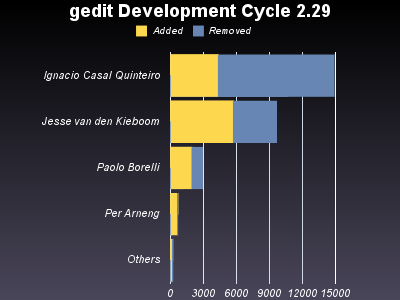
\includegraphics[scale=0.45]{./images/gedit-development-2-29}
    \caption{gedit development 2.29}
  \end{minipage}
  \hspace{0.5cm}
  \begin{minipage}[b]{0.5\linewidth}
    \centering
    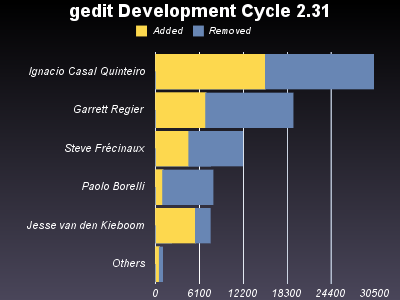
\includegraphics[scale=0.45]{./images/gedit-development-2-31}
    \caption{gedit development 2.31}
  \end{minipage}
\end{figure}

Just point out that this cycle has been particularly hard for application developers, especially those that try to adopt early, so that they are actually ready by the time GNOME 3.0 lands. And then to think, for the end user, there will be basically no change at all...
